\section{Development}

\subsection{Introduction}
In this section, I will discuss the development process of the domain project.  There will be six sections, each exploring the six main features established in the requirement section, which are declaration of domains, assignment of signatures to function/methods, declaration of variables, combination of domains, implicit conversions of variables, and type checking at compile time. 

\subsection{Declaration of domains}
The first feature  I have implemented was declaration of domains.  There are several methods and classes that are relevant to the code, which will be discussed one by one.  
\begin{lstlisting}[caption={Method for creating domains}]
def create_domain(compound: 0, name: "")
    if !block_given? && compound == 0
        raise ArgumentError.new "No block of rules were given.  There must be at least one rule for the domain"
    end

    cl = Class.new do
       extend DomainClass   
        include DomainClass
    end

    prev = @domain_created

    @domain_created = cl

    @domain_created.compound_domain = unless compound == 0 then compound else @domain_created end
    @domain_created.rules = {}
    @domain_created.translators = {}
    @domain_created.default = nil
    @domain_created.translation_map = {}

    yield if block_given?
        
    @domain_created.translators.each_key do |key|
        d_in, d_out = key

        if !@domain_created.translation_map.has_key? d_in
            @domain_created.translation_map[d_in] = []
        end

        @domain_created.translation_map[d_in] << d_out
    end

    @domain_created = prev

    cl.send :generate_translators

    if not name.empty?
        if self.inspect == 'main'
            Object.const_set(name, cl)
        else
            self.const_set(name, cl)
        end
    else
        return cl
    end
end
\end{lstlisting}

The first of the relevant methods is create\_domain.  This method is simple compared to some of the TracePoint driven methods that will appear in the later codes.  First, the code checks to see if there are any rules with the provided domain.  This is done to prevent users from create a domain that lacks any rules.  Next, the method creates an anonymous class that implements DomainClass, which is a module that contains various basic functions for domains to function, which will be shown in Figure 2. Next, an instance varialbe @domain\_created is stored in prev variable.  This is because the @domain\_created variable is basically a global variable for the create\_domain method, and if another domain was declared within the block, the value can be overridden with the new domain.  To prevent this, prev store the value @domain\_created was previously and return it to the original value after the domain is created.  After prev has been set, the anonymous class is assigned to @domain\_created and all important values such as rules and translation rules are initiated.  The block is then yielded to read all the rules inside, and saved to the hashes. The lines 23 to 35 will be explained in detail in the later sections, as it is more relevant there.  Finally, the anonymous class is given a name and is defined in the appropriate classes as a constant. 

\begin{lstlisting}[caption={Domain module}]
module DomainClass
    include DomainErrors
    attr_accessor :rules
    attr_accessor :translators
    attr_accessor :compound_domain
    attr_accessor :default
    attr_accessor :translation_map

    def print_rules; end

    def print_translators; end

    def value?(value); end

    def check_rules(rules, value); end

    def translate(d_in, d_out, value); end

    def value=(value); end

    def value(domain=nil); end
end
\end{lstlisting}

DomainClass module is the next set of codes that will be discussed.  This module contains various different methods a domain should have to function properly.  The implementations for each of the methods are omitted to prevent codes from taking too much space and because they are mostly self-explanatory.  The most important methods are value?, value=, and value.  value? method checks the value in the argument to make sure the argument follows the rules of the domain.  check\_rules in the module is the private helper method for the value? method.  value= assigns the value to the domain for domain to use in the future, which can be read through the value method.  Domain should also have ways to translate from one domain to another, which is used in implicit conversions.

\begin{lstlisting}[caption={Monkey patching Object class}]
class Object
    class << self
        include Util
        def rules
            [{ self => Proc.new { |x| true } }]
        end

        def compound_domain
            self
        end

        def translators
            {}
        end

        def value?(x)
            return x.is_a? self
        end

        def has_compound_domain
            self != compound_domain
        end

        def method_added(m)
            super
        end

        def singleton_method_added(m)
            super
        end

        make_compound_domain :+
        make_compound_domain :-
        make_compound_domain :&

        alias :union :+
        alias :intersect :&
        alias :difference :-
    end

    def part_of?(x)
        if x.singleton_methods.include? :value?
            x.value? self
        end

        raise TypeError.new("#{x} is not a domain.")
    end

    def value
        return self
    end
end
\end{lstlisting}

Finally, the domain adds new methods to Object class so that all class behave similarly to the domains, as type is a subset of domain in type checking sense.  This allows classes that already exist, such as Integer and String class, act similarly to the domain, which allows the program to treat them like one for various benefits such as the combination of domains.

Through these methods, the users of this library can create domain using syntax like this:

\begin{lstlisting}[caption={Sample code: declaration of domains}]
def is_integer(x)
    return Integer(x) rescue false
end

domain :Int do
    rule(Integer)
    rule(String) { |x| is_integer?(x) }
end
\end{lstlisting}

The domain :Int do \ldots end defines domain Int with two rules.  The first rule states that it can accept any Integer, and the second rule states that if the object is String, domain Int can accept values that returns true for the is\_integer?() method, which checks if the x is an integer.  With this domain, it is possible to use both integer and string only containing integer as if they're integer, which can be a very power tool.

\subsection{Assignment of signatures to function/methods}

Unlike the declaration of domain, the implementation of signatures require heavy exploitation of Ruby's metaprogramming features, which can be difficult to understand.  Additionally, the implementation is very long, so it requires extensive explanation on how they are implemented.

The signature is implemented in three steps.  First, the signature reads the String passed in as a signature and parse and interpret the string to see if the String is a valid signature.  The string is then transformed into two arrays, each indicating the rules for argument and rules for return values respectively.  The arrays are then used to wrap the new method with checks that makes sure the argument and return value conforms to the rules and the original method is overridden with the new wrapped method.  We will discuss each parts in detail over this section

\begin{lstlisting}[caption={Parser method}]
def parse_tokens(sig)
    valid_tokens = ['(', ')', ',', '[', ']', '$', '{', '}', '&']
    sig.gsub!(/\s/, "")

    tokens = []

    other = ""
    token = ""

    state = :default
    redo_state = false

    sig.each_char do |x|
        case state
        when :default
            token += x
            case x
            when '*'
                state = :star
            when '-'
                state = :arrow
            when *valid_tokens
                state = :accepted
            else
                state = :other
            end
        when :star
            case x
            when '*'
                state = :accepted
                token += x
            else
                state = :accepted
                redo_state = true
            end
        when :arrow
            token += x
            case x
            when '>'
                state = :accepted                   
            else
                state = :other
            end
        end

        if state == :other
            other += token
                
            if token == ":" then state = :accepted else state = :default end
            token = ""
        end
            
        if state == :accepted
            if !other.empty? then tokens << other; other = "" end
            tokens << token if !token.empty?
            token = ""
            state = :default
        end

        if redo_state
            state = :default
            redo_state = false
            redo
        end
    end

    tokens << other if !other.empty?
    tokens
end
\end{lstlisting}

First, this method parses the string into list of tokens that can be used to interpret what it means.  The method follows the following finite state machine to parse the string:

\begin{figure}[h]
\caption{Finite State Machine}
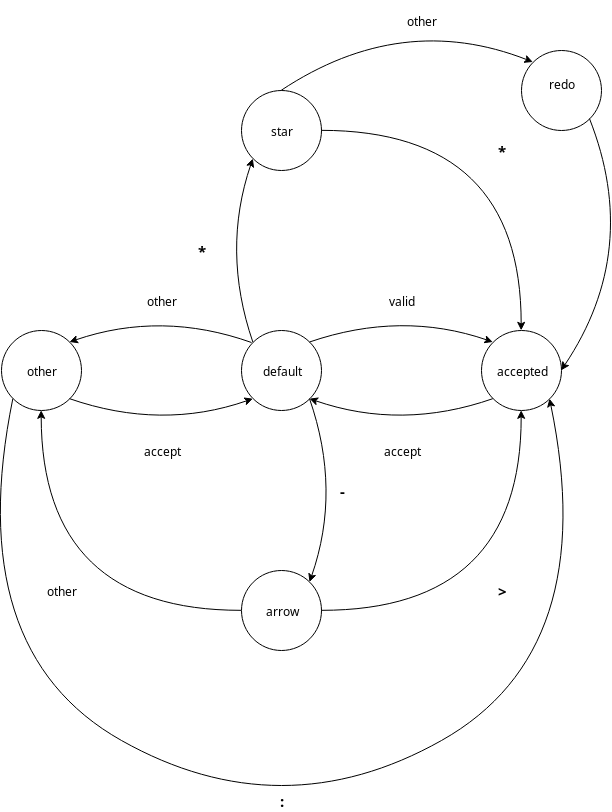
\includegraphics[width=10cm]{diagram_fsm}
\centering
\end{figure}

The machine begins at default, and moves to star state when it finds a {*} symbol, arrow state ({-}\textgreater) when it finds the {-} symbol, accepted state when it finds any of the valid tokens defined in the array, and other state for any other symbols.  On star state, it moves to accepted state when it finds another {*} symbol and redo state otherwise, which is a state that quickly moves to accepted state and re-examine the current symbol.  The arrow state changes to accepted state only when it finds the \textgreater symbol which completes the arrow.  The remaining other symbols move to other state.  Other state simply concatenates the value to a variable, and if {:} was found, Other moves to accepted state to save it as a keyword.  On accepted state, the tokens that has been found is stored in an array.  After the entire string has been parsed, the array is returned.

\begin{lstlisting}[caption={Interpreter method}]
def interpret_tokens(cl, local, tokens)
    # Get tokens for arg and return separated

    k = tokens.slice_after { |x| x == '->' }.to_a
    a, r = k
    a.pop
    length = k.length

    if length != 2
        raise ArgumentError.new "Expected only one arrow (->), got #{length - 1}"
    end

    # Change the list of tokens into something more usable

    # Ignore the () if it's properly at the begnning and end
    a = a[1..-2] if a[0] == '(' && a[-1] == ')'
    r = r[1..-2] if r[0] == '(' && r[-1] == ')'

    a = retrieve_tokens(cl, local, a)
    r = retrieve_tokens(cl, local, r)[0]

    return a, r
end
\end{lstlisting}

Now that all the tokens are in array, the next step is to store them into two arrays, one for argument and another for return values.  Once the tokens are separated, it is sent to retrieve token method, which will turn all the tokens into something the wrapper can use to check the values.

\begin{lstlisting}[caption={Retriever method}]
def retrieve_tokens(cl, local, tokens)
    # initialization

    tokens.each do |x|
        case state
        when :token
            case x
            when '['
                # array logic
            when '{'
                # hash logic
            when ',', ']', '}'
                # error
            when '*', '**'
                # star logic
            when '$'
                # optional logic
            when '&'
                # block logic
            else
                # non-token logic
        when :comma
            # comma logic
        end
    end
    return arg, kwarg
end
\end{lstlisting}

The retrieve\_token method can be generalized through this code.  After initializing important variables, the method iterates through all the tokens that are given, and performs different checks to see what the token means.  There are two states in this method, which are ``token'' and ``comma''.  Because the tokens alternate between valid token and comma in real code, this two states are alternated between each other to make sure all tokens separated by comma means something.

\begin{lstlisting}[caption={Wrapper method: overview}]
def wrap_method(signature)
    # initialize

    return_trace = TracePoint.new(:return) do |tp|
        # parse signature
	# initialization for the new method
	# check if the method has correct argument(s)
	# wrap the method with checks and replace it
	# add it to the correct place and with right scope
    end

    line_trace = TracePoint.trace(:line) do |tp|
    	# get a binding
	# enable return_trace and disable line_trace
    end
end
\end{lstlisting}

Next, the wrapper method uses the established parser in order to wrap the method correctly.  Because this method is large, all logic will be separated into multiple sections to explain them all in detail.

\begin{lstlisting}[caption={Wrapper method: check if the method has correct argument(s)}]
return_trace = TracePoint.new(:return) do |tp|
    # ...
    # Check for validity of the method by getting its arity and aligning it with the length of arguments in signature
    method = tp.self.instance_method(method_name) if tp.method_id == :method_added
    method = tp.self.method(method_name) if tp.method_id == :singleton_method_added

    # Check if the parameters should have star variable (*arg) or double star variable (**arg)
    has_star = false
    has_dstar = false

    args.each do |x|                        
        has_star = true if is_star?(x) && x.star == '*'
        has_dstar = true if is_star?(x) && x.star == '**'
    end

    has_dstar = !kwargs.empty? unless has_dstar

    # Get all the parameters for the method
    param = method.parameters

    # initialization
    optional_arg = []
    optional_kwarg = []
    expected_length_arg = 0
    expected_length_kwarg = 0

    # args is nil, so there should not be any parameters except for the blocks
    if args.length == 1 && args[0].nil? && param.reject{ |x| x[0] == :block }.length == 0
        next
    else
        # Then see if the variables are structured properly, such as making sure that star variable is a 3rd variable if the signature also have star variable for 3rd
        param_arg = param.reject { |x| x[0] != :req && x[0] != :opt && x[0] != :rest }
        if param_arg.length != args.length
            raise SignatureViolationError.new "Wrong number of total arguments: Expected #{args.length}, found #{param_arg.length}"
        end
        # Iterate every rules
        args.zip(param).each_with_index do |x, i|
            ar, par = x

            # Check if the parameter is what we expected
            case
            when ar.class == Class
                if par[0] != :req
                    raise SignatureViolationError.new "Expected a required variable for #{par[1]}, found #{par[0]}"
                end
                expected_length_arg += 1
            when is_star?(ar)
                if par[0] != :rest
                    raise SignatureViolationError.new "Expected a * variable for #{par[1]}, found #{par[0]}"
                end
            when is_optional?(ar)
                optional_arg << i
                if par[0] != :opt
                    raise SignatureViolationError.new "Expected an optional variable for #{par[1]}, found #{par[0]}"
                end
                expected_length_arg += 1
            end
        end

        # Do the same thing for the keyword section
        key_matched =  []

        param_kwarg = param.reject { |x| x[0] != :keyreq && x[0] != :key}
        if param_kwarg.length != kwargs.length
            raise SignatureViolationError.new "Wrong number of keyword arguments: Expected #{kwargs.length}, found #{param_kwarg.length}"
        end
                
        param.each do |par|
            if kwargs.has_key?(par[1])
                key_matched << par[1]
                if is_optional?(kwargs[par[1]])
                    optional_kwarg << par[1]
                end
            end
        end

        missing = kwargs.keys - key_matched
        missing = [] if has_dstar

        if !missing.empty?
            raise SignatureViolationError.new "The following keywords are not in the argument: #{missing}"
        end
    end
    # ...
end
\end{lstlisting}

The second step in wrapping method is to determine if the method given has the right argument at the right area:

\begin{lstlisting}[caption={Example: wrapper method}]
# error, first argument should be required, and second should be optional
domain 'String, $String -> nil'
def f(x = 5, y)
end

# no error
domain 'String, $String -> nil'
def f(x, y = 5)
end
\end{lstlisting}

As evident by this example, the first method f does not follow the rules provided.  The signature stated that the first argument is required while second argument is optional, yet the f provides the opposite.  Additionally, there can be too much or too little arguments on f that would break the rule.  To prevent this type of rule breaking, this part of wrapper goes through all the parameters of the method and the rules for the argument and check if they match.

\begin{lstlisting}
return_trace = TracePoint.new(:return) do |tp|
    # ...
    # wrap the method
    lamb = lambda do
        tp_self.send use, method_name do | *arg1, **arg2, &block |
            old_arg1 = arg1
            old_arg2 = arg2

            all_args = [pad_with_optional(arg1, optional_arg, expected_length_arg), arg2]
            arg_types = args
            kwarg_types = kwargs

            if has_star
                check_array all_args[0], arg_types
            else
                (all_args[0].zip(arg_types)).each do |arg_type|
                    arg, type = arg_type

                    check_validity arg, type
                end
            end

            check_keyword all_args[1], kwarg_types

            if arg1.length == 0 && arg2.length == 0
                r = self.send(old_method_name) { block.call } if !block.nil?
                r = self.send(old_method_name) if block.nil?
            elsif arg2.length == 0
                r = self.send(old_method_name, *old_arg1) { block.call } if !block.nil?
                r = self.send(old_method_name, *old_arg1) if block.nil?
            elsif arg1.length == 0
                r = self.send(old_method_name, **old_arg2) { block.call } if !block.nil?
                r = self.send(old_method_name, **old_arg2) if block.nil?
            else
                r = self.send(old_method_name, *old_arg1, **old_arg2) { block.call } if !block.nil?
                r = self.send(old_method_name, *old_arg1, **old_arg2) if block.nil?
            end

            all_rets = if r.is_a?(Enumerable) then r else [r] end
            ret_types = if ret.is_a?(Enumerable) then ret else [ret] end

            all_rets.zip(ret_types).each do |ret_type|
                ret, type = ret_type
                        
                check_validity ret, type
            end

            all_rets
        end
    end
    # ...
end

\end{lstlisting}

\subsection{Declaration of variables}

\begin{lstlisting}[caption={Method for calling define initializer correctly}]
def create_initializer(a, domain)
    line = 0

    tp = TracePoint.trace(:line) do |x|
        line += 1

        if line == 2
            bind = x.binding

            if x.self.inspect != "main"
                x.self.class_eval do
                    DomainCreate::define_initializer a, domain
                end
            else
                Object.class_eval do
                    DomainCreate::define_initializer a, domain
                end
            end

            x.disable
        end
    end
end
\end{lstlisting}

\begin{lstlisting}[caption={Method for defining the initializer method}]
def define_initializer(a, domain)
    define_method a do |sym|
        layer = 1
        bind = nil
        obj_id = 8
        line_checked = 0
        path_checked = 0

        line_trace = TracePoint.trace(:line) do |x|
            if bind != nil
                new_obj_id = 0
                value = bind.local_variable_get(sym) if bind.local_variable_defined?(sym)
                new_obj_id = value.object_id if bind.local_variable_defined?(sym)

                if new_obj_id != obj_id && line_checked != 0 && path_checked != 0
                    if !domain.value? value
                        raise ValueOutOfBoundsError.new "from #{path_checked}:#{line_checked}: '#{value}' assigned to variable '#{sym}', which is out of bounds from '#{domain.name}'"
                    end

                    val = domain.new
                    val.value = value

                    bind.local_variable_set(sym, val)
                end

                obj_id = new_obj_id

                path_checked = x.path
                line_checked = x.lineno
            else
                next
            end
        end

        call_trace = TracePoint.trace(:call) do |x|
            line_trace.disable if line_trace.enabled?

            layer += 1
        end


        return_trace = TracePoint.trace(:return) do |x|
            layer -= 1

            if layer == 0
                line_trace.enable
            end

            if layer == -1
                line_trace.disable
                x.disable
                call_trace.disable
            end
        end

        bind_trace = TracePoint.trace(:line) do |x|
            bind = x.binding
            bind_trace.disable
        end
    end
end
\end{lstlisting}
\subsection{Combination of domains}

\subsection{Implicit conversion of variables}

\subsection{Type Checking at Compile Time}
